\chapter{はじめに}

\section{研究背景}
本研究の背景には,ニューラルネットワークを用いた深層学習と格子ボルツマン法(Lattice Boltzmann Method, LBM)の二つの重要な要素がある.一方の深層学習は機械学習の一分野であり,複数の隠れ層を持つニューラルネットワークを使って複雑なパターンを学習する手法である\cite{doi:10.1126/science.1127647}.近年盛んに研究されていて応用先の一つに気象予測があり\cite{Schultz2021},例えばCNN(Convolutional Neural Network)\cite{Yamashita2018}とLSTM(Long Short-Term Memory)\cite{10.1162/neco.1997.9.8.1735}を用いた正方形領域での風速予測がされている\cite{CHEN2021114451}.他方で,格子ボルツマン法は1990年代以降に発展した比較的新しい数値流体力学の手法であり,個々の粒子のふるまいを扱うのではなく,格子状に分割した空間内で各格子点上の離散化された速度分布関数を解くものである\cite{doi:10.1146/annurev.fluid.30.1.329}.この手法の長所として並列計算と相性がよいことが挙げられ,GPUやTPUのようなプロセッサ上で効率的に計算することができる\cite{Satofuka1999}.これはニューラルネットワークにも共通する特性である\cite{OH20041311}.

\section{先行研究}
\subsection{CNNとLSTMを用いた正方形領域での風速予測 \label{subsec:chen2021}}
Chenら(2021)は,CNNとLSTMを用いたモデルによる正方形領域での風速予測を行った\cite{CHEN2021114451}.彼らのモデル概要図を図\ref{fig:chen2021_architecture}に示す.この図において,エンコーダとデコーダの部分にCNNが用いられており,これにより正方形領域における格子点上の風速の空間的なパターンを学習している.また,エンコーダの出力をLSTMに入力し,更にその出力をデコーダに入力している.このLSTMのユニットにより,時間的なパターンも学習している.
\begin{figure}[bp]
    \centering
    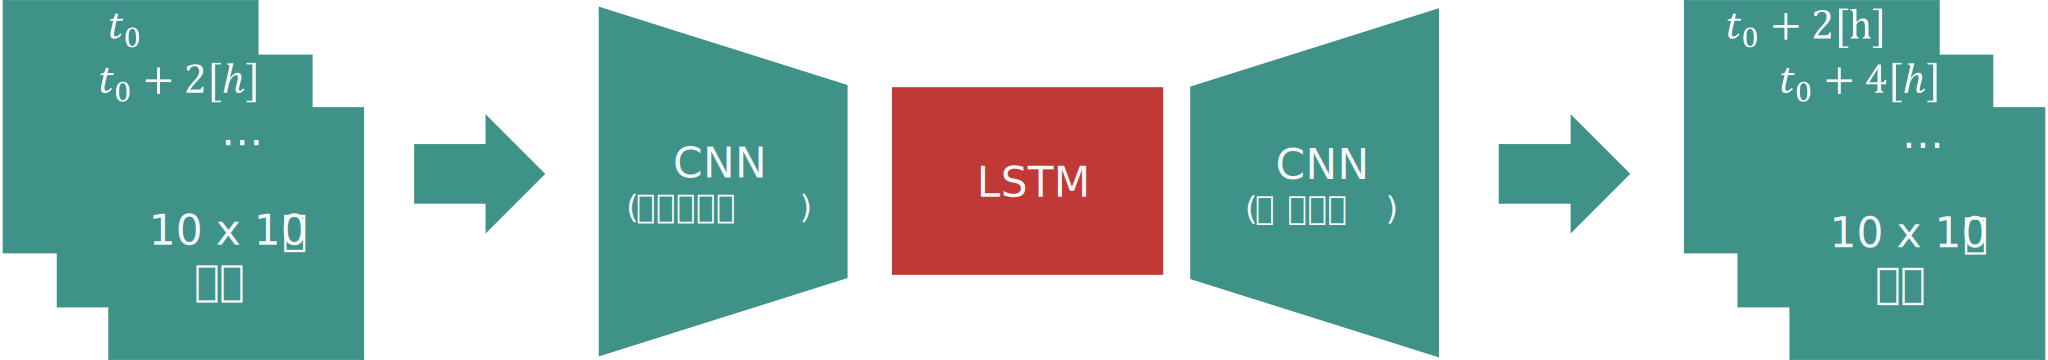
\includegraphics[width=0.9\textwidth]{./introduction/figs/chen2021_model_overview.svg.eps}
    \caption{Chenら(2021)のモデル概要図\cite{CHEN2021114451}}
    \label{fig:chen2021_architecture}
\end{figure}

このモデルを使って,彼らは図\ref{fig:chen2021_region}に示すようにアメリカのインディアナ州内部で,2km間隔の$10 \times 10$格子点上で2時間先の風速予測を行い,単にANN(Artificial Neural Network)\cite{485891}やLSTMのみを用いたモデルに比較して精度が向上することを示した.具体的には,全体の風速予測の平均絶対誤差(Mean Absolute Error, MAE)が$0.35 \mathrm{m/s}$減少し,これはPersistence モデル,ANNのみのモデル, LSTMのみのモデルの結果に比べてそれぞれ$32.7\%$, $28.8\%$, $18.9\%$低い値であると主張している.ここで,Persistence モデルとは,風速の時間変化を考慮せず,直前の風速をそのまま予測値とするモデルである.
\begin{figure}[bp]
    \centering
    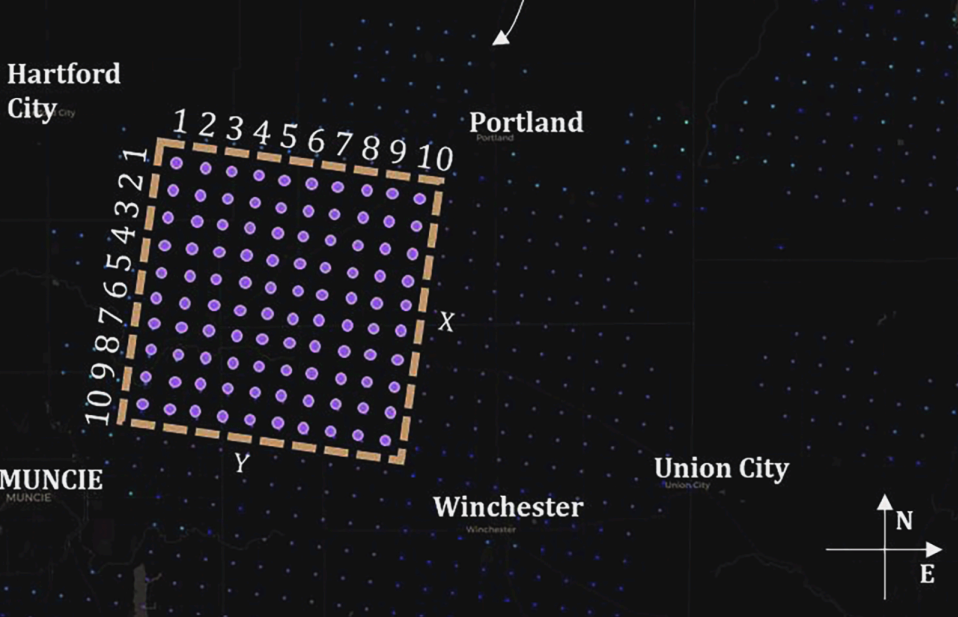
\includegraphics[width=0.8\textwidth]{./introduction/figs/chen2021_region.png.eps}
    \caption{Chenら(2021)が風速予測を行った範囲\cite{CHEN2021114451}}
    \label{fig:chen2021_region}
\end{figure}

\subsection{Physics-Informed Neural Networks}
Raissi(2020)らは,物理学の知識をニューラルネットワークに組み込むことで,データが少ない場合でも高精度な予測を行うことができるPhysics-Informed Neural Networks(PINNs)というモデルを提案した\cite{PINNs2020}.このモデルは流体のシミュレーションに使われることが多く\cite{app13126892},ここでもその用途を想定する.彼らの提案したモデル概要図を図\ref{fig:pinns-overview}に示す.
\begin{figure}[bp]
    \centering
    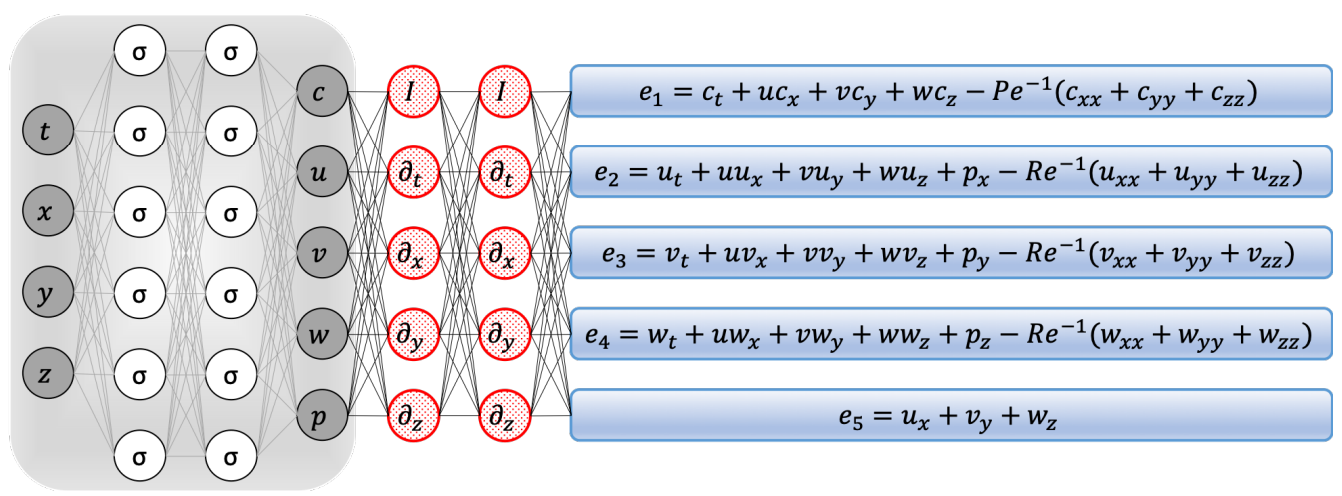
\includegraphics[width=0.9\textwidth]{./introduction/figs/PINNs_overview.png.eps}
    \caption{Raissiら(2020)のモデル概要図\cite{PINNs2020}}
    \label{fig:pinns-overview}
\end{figure}
この図が示すように,彼らのモデルは座標$x$,$y$,$z$と時刻$t$を入力とし,それに対応する流体のパッシブスカラーの濃度$c$,流体の速度$u$,$v$,$w$,そして流体の圧力$p$を出力する.なおパッシブスカラーとは,流体の流れによって変化するが流体の流れに影響を与えない物理量のことであり,例えば流体に溶けた微量な染料の濃度などが挙げられる\cite{Lesieur1990}.

彼らのモデルは,損失関数(\ref{subsection:neuron-principles}項参照)に物理的な微分方程式からどれだけモデルの出力が乖離しているかを表す項を組み込むことで,物理法則を満たすように学習をする.図\ref{fig:pinns-overview}中では$e_1$,$e_2$,$e_3$,$e_4$,$e_5$がこの項に当たる.このとき,物理量の座標微分や時間微分は,\ref{subsection:automatic-differentiation}項に述べるように自動微分を使って導くことができる.実測データが少ない場合でも,それ以外の座標と時刻を入力した場合の損失が小さくなるようにすれば,モデルは物理法則に従うと彼らは主張している.

%この手法では,物理的な外力や拘束条件が既知の場合では有効であるが,例えば大気のように外力や拘束条件が不明または特定が困難な場合には損失関数をどう定めればよいのかわからず,適用するのが難しいという問題点がある. %これは良くない気がする.なぜなら,そもそもデータセットが少ない場合に適応するのが目的だから,データセットが多い場合はそもそもPINNsを使う必要がないから




\section{研究目的}
本研究では\ref{subsec:chen2021}項で述べたChenら(2021)の研究と同様に,長方形領域における格子点上での風速予測を行うが,ニューラルネットワークの構造にLBMを組み込むことで,LBMの持つ並列計算と相性の良さを活かしつつ,精度の向上を図る.

本研究はデータセットが十分あるが,大気の動きのように外力や拘束条件が不明または特定が困難な場合にも,物理法則を利用できるモデルを提案することを目的としている(PINNsと比較して).% todo: この辺推敲
% todo: 結果とか考察を加味して後で加筆修正,その際に修論概要書と整合性をとる
% todo: 先行研究との位置づけで,PINNsとは違うやり方で物理法則を組み込むよ,みたいなことも触れる
% todo: 地球の球体性を考慮するとかも書く

\section{論文構成}
本論文では,第\ref{section:deep-learning}節で深層学習の,第\ref{section:lbm}節で格子ボルツマン法の数理的な原理を解説し,それらを踏まえて第\ref{chap:how-to-assemble}章で提案モデルでは格子ボルツマン法をどのように深層学習モデルに組み込んだのかを解説する.第\ref{chap:experiments}章では,提案モデルの有効性を検証するため,日本近辺の風速予測を行い,従来研究のモデルと比較検討をする.